%% This is file `elsarticle-template-1-num.tex',
%%
%% Copyright 2009 Elsevier Ltd
\documentclass[final,3p]{elsarticle}

\usepackage{lipsum}
\makeatletter
\def\ps@pprintTitle{%
 \let\@oddhead\@empty
 \let\@evenhead\@empty
 \def\@oddfoot{}%
 \let\@evenfoot\@oddfoot}
\makeatother

%% Use the option review to obtain double line spacing
%% \documentclass[preprint,review,12pt]{elsarticle}

%% Use the options 1p,twocolumn; 3p; 3p,twocolumn; 5p; or 5p,twocolumn
%% for a journal layout:
%% \documentclass[final,1p,times]{elsarticle}
%% \documentclass[final,1p,times,twocolumn]{elsarticle}
%% \documentclass[final,3p,times]{elsarticle}
%% \documentclass[final,3p,times,twocolumn]{elsarticle}
%% \documentclass[final,5p,times]{elsarticle}
%% \documentclass[final,5p,times,twocolumn]{elsarticle}

%% The graphicx package provides the includegraphics command.
\usepackage{graphicx}
%% The amssymb package provides various useful mathematical symbols
\usepackage{amssymb}
%% The amsthm package provides extended theorem environments
%% \usepackage{amsthm}

%% The lineno packages adds line numbers. Start line numbering with
%% \begin{linenumbers}, end it with \end{linenumbers}. Or switch it on
%% for the whole article with \linenumbers after \end{frontmatter}.
\usepackage{lineno}

%% natbib.sty is loaded by default. However, natbib options can be
%% provided with \biboptions{...} command. Following options are
%% valid:

%%   round  -  round parentheses are used (default)
%%   square -  square brackets are used   [option]
%%   curly  -  curly braces are used      {option}
%%   angle  -  angle brackets are used    <option>
%%   semicolon  -  multiple citations separated by semi-colon
%%   colon  - same as semicolon, an earlier confusion
%%   comma  -  separated by comma
%%   numbers-  selects numerical citations
%%   super  -  numerical citations as superscripts
%%   sort   -  sorts multiple citations according to order in ref. list
%%   sort&compress   -  like sort, but also compresses numerical citations
%%   compress - compresses without sorting
%%
%% \biboptions{comma,round}

% \biboptions{}

\journal{STAT 578}

\date{}


% ---------------------------------------------------------------------
\begin{document}

\begin{frontmatter}

%% Title, authors and addresses

\title{Large Scale Landmark Recognition via Deep Learning}

%% use the tnoteref command within \title for footnotes;
%% use the tnotetext command for the associated footnote;
%% use the fnref command within \author or \address for footnotes;
%% use the fntext command for the associated footnote;
%% use the corref command within \author for corresponding author footnotes;
%% use the cortext command for the associated footnote;
%% use the ead command for the email address,
%% and the form \ead[url] for the home page:
%%
%% \title{Title\tnoteref{label1}}
%% \tnotetext[label1]{}
%% \author{Name\corref{cor1}\fnref{label2}}
%% \ead{email address}
%% \ead[url]{home page}
%% \fntext[label2]{}
%% \cortext[cor1]{}
%% \address{Address\fnref{label3}}
%% \fntext[label3]{}


%% use optional labels to link authors explicitly to addresses:
%% \author[label1,label2]{<author name>}
%% \address[label1]{<address>}
%% \address[label2]{<address>}

\author{Jifu Zhao}

\address{Department of Nuclear, Plasma, and Radiological Engineering \\
University of Illinois at Urbana-Champaign, Urbana, Illinois 61801, USA}

\ead{jzhao59@illinois.edu}
\ead[]{All code is available in GitHub: https://github.com/JifuZhao/Landmark-Recognition}

% ---------------------------------------------------------------------
\begin{abstract}
%% Text of abstract
Landmark recognition is one kind of object recognition problem that hasn't been well solved. Due to large number of landmarks and highly imbalanced dataset, the classical methods used for object recognition cannot be directly applied. This paper presents the application of triplet network for large scale landmark recognition. Through fine-tuning pretrained convolutional network network (CNN) and minimizing triplet loss, the triplet network can learn appropriate metric such that most similar images can be retrieved through k-nearest neighbor (KNN) algorithms. The performance of the proposed method is evaluated on real-world landmark recognition dataset.
\end{abstract}

% ---------------------------------------------------------------------
\begin{keyword}
%% keywords here, in the form: keyword \sep keyword
Landmark recognition \sep Triplet network \sep Deep learning \sep Metric learning
\end{keyword}

\end{frontmatter}

%%
%% Start line numbering here if you want
%%
%\linenumbers

% ---------------------------------------------------------------------
\section{Introduction}
\label{S:introduction}

Over the recent years, with the rapid development of deep learning techniques, especially convolutional neural networks (CNN), people have achieved huge progress in computer vision. Different kinds of network architectures have been proposed. Some widely used architectures include VGG~\cite{simonyan2014very}, ResNet~\cite{he2016deep}, Inception Network~\cite{szegedy2016rethinking} and so on. On the famous ImageNet Large Scale Visual Recognition Challenge (ILSVRC), some algorithms have achieved higher accuracy than human beings. 

CNNs have been proven to be one of the best solutions for computer vision tasks, which have been widely used in different areas, such as autonomous cars and automatic face recognition. The fast development of deep learning and computer vision techniques have changed people's lifestyle. However, classical object recognition tasks generally require large amount of training images. For example, CIFAR-10 dataset~\cite{krizhevsky2009learning} contains 60,000 training images in 10 different classes. ImageNet dataset~\cite{imagenet_cvpr09} contains 14,191,122 images in 1,000 classes. Large amount of training images is one of the key factors to guarantee the success of CNNs. In addition, object recognition systems usually use fully-connected layer as the structure for the final one or several layers, which typically requires large amount of parameters. 

However, there exists a special kind of problem called one-shot learning~\cite{fei2006one} that cannot be easily solved with the classical methods. One-shot learning aims to learn information from one, or only a few, training images. And there could be a huge amount of classes. These two factors require new solutions. There are several famous one-shot learning examples, such as face recognition/verification and famous street-to-shop~\cite{liu2012street} systems. Over the past several years, a series of solutions have been proposed to solve one-shot learning problems. For example, Siamese network~\cite{koch2015siamese} has been proposed for different problems including authorship and image recognition. Face recognition or face verification have been well studied~\cite{schroff2015facenet, liu2015targeting}. Triplet-based networks have been studied for audio and image retrieval problems~\cite{wang2014learning, lin2015rapid, kiapour2015buy, wang2016matching, shankar2017deep, qi2017audio}

This paper focuses on landmark recognition from images. There are thousands of landmarks exist. Some are very popular and some are less popular. People around the world take countless photos that contain different landmarks, which provide enough training images. Due to highly imbalanced dataset and large amount of different landmarks, this paper focuses on one-shot learning for landmark recognition. More specifically, with some reference images that contain different landmarks, given a new image, this paper wants to design an algorithm that can automatically detect the landmarks the new image contains. Fig.~\ref{fig:problem} shows an illustration of the landmark recognition problem.

% ---------------------------------------------------------------------
\begin{figure}[hbtp]
\centering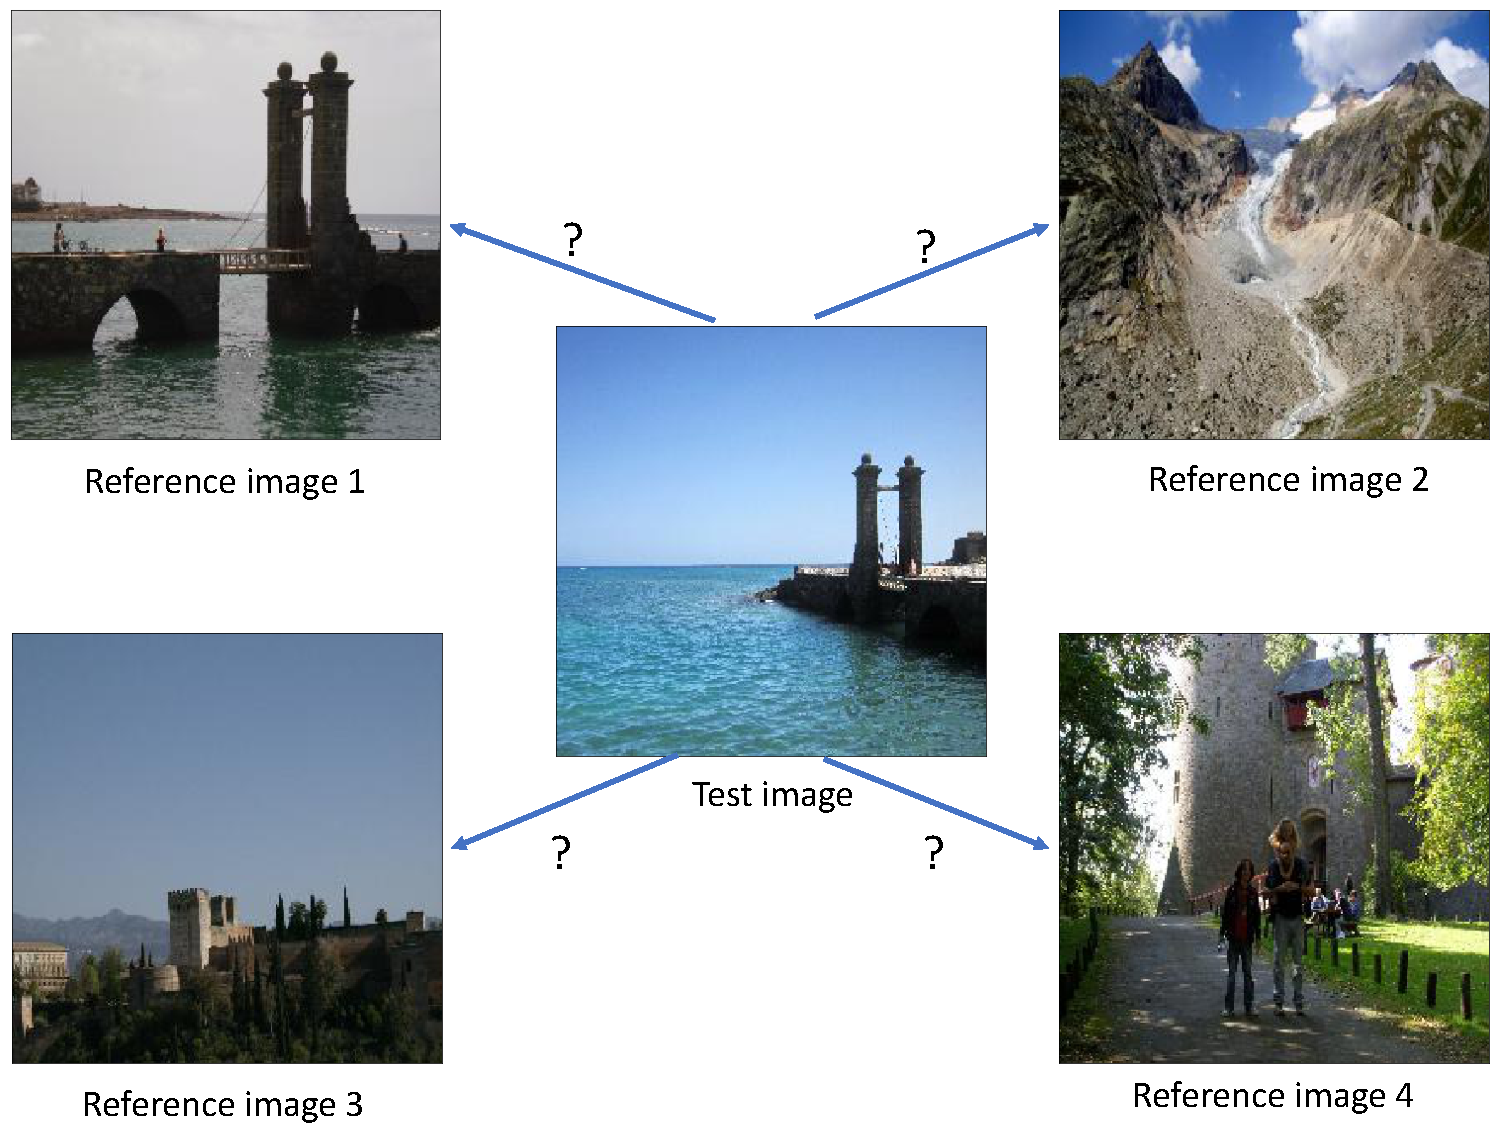
\includegraphics[width=0.8\linewidth]{./figures/problem.pdf}
\caption{Illustration of landmark recognition problem}
\label{fig:problem}
\end{figure}

% ---------------------------------------------------------------------
\section{Data}
\label{S:data}

For a successful landmark recognition system, training data are very important. Large amount of training images that contain as many different landmarks as possible can help build more robust systems. The data used in this work come from Google-Landmarks dataset, which is released by Google on early March 2018. The whole Google-Landmarks dataset contains human-made and natural landmarks across the world. There are 1,225,029 training images in 14,951 different landmarks. A subset of 12 randomly sampled images are shown in Fig.~\ref{fig:sample}.

% ---------------------------------------------------------------------
\begin{figure}[hbtp]
\centering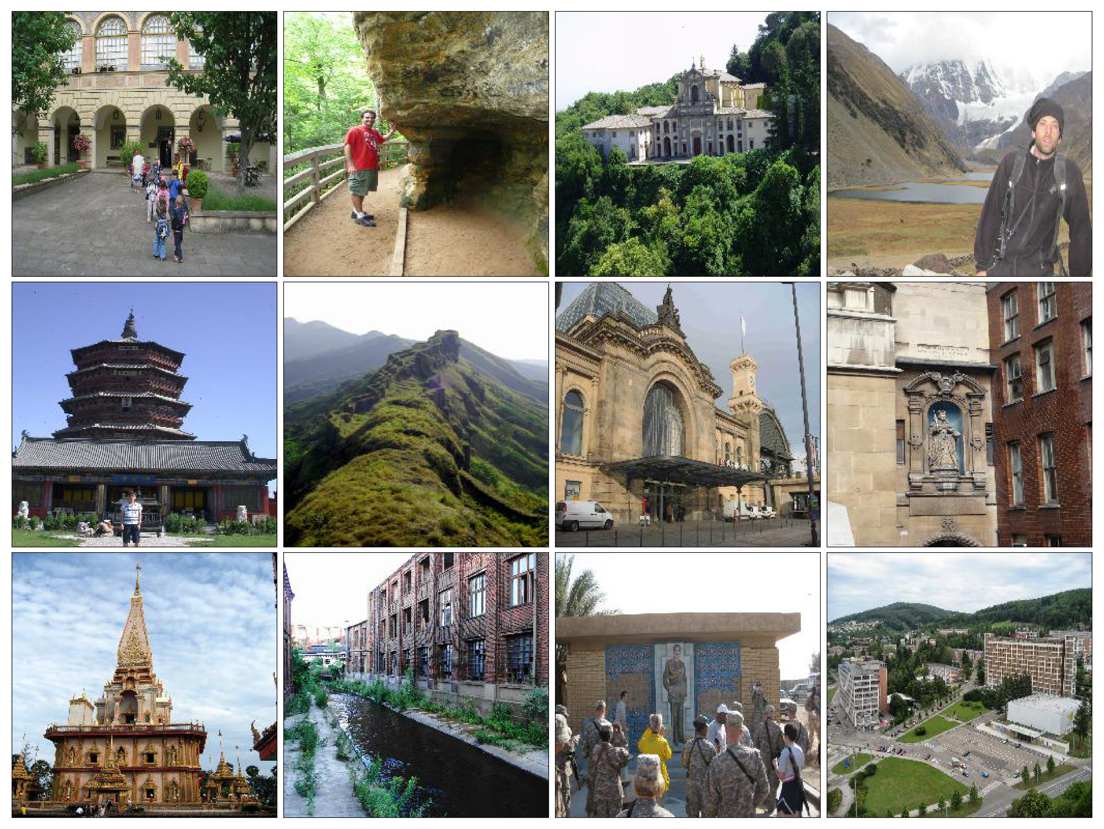
\includegraphics[width=0.94\linewidth]{./figures/sample.png}
\caption{Subset of sample images}
\label{fig:sample}
\end{figure}

As shown in Fig.~\ref{fig:sample}, the training images are pretty noisy. The landmarks may not be at the center of the whole image and some landmarks might be blocked by humans. All these factors make it quite challenging. Fig.~\ref{fig:all_distribution} shows the count distribution of different landmarks sorted by the number of images for each landmark. It is clear that for some popular landmarks, such as Eiffel Tower and Mount Fuji, there are large amount of training images available. For example, the most popular landmarks contain more than 5,000 images. However, for less popular landmarks, the available images are few, and some landmarks only have one image. 

% ---------------------------------------------------------------------
\begin{figure}[htbp]
\centering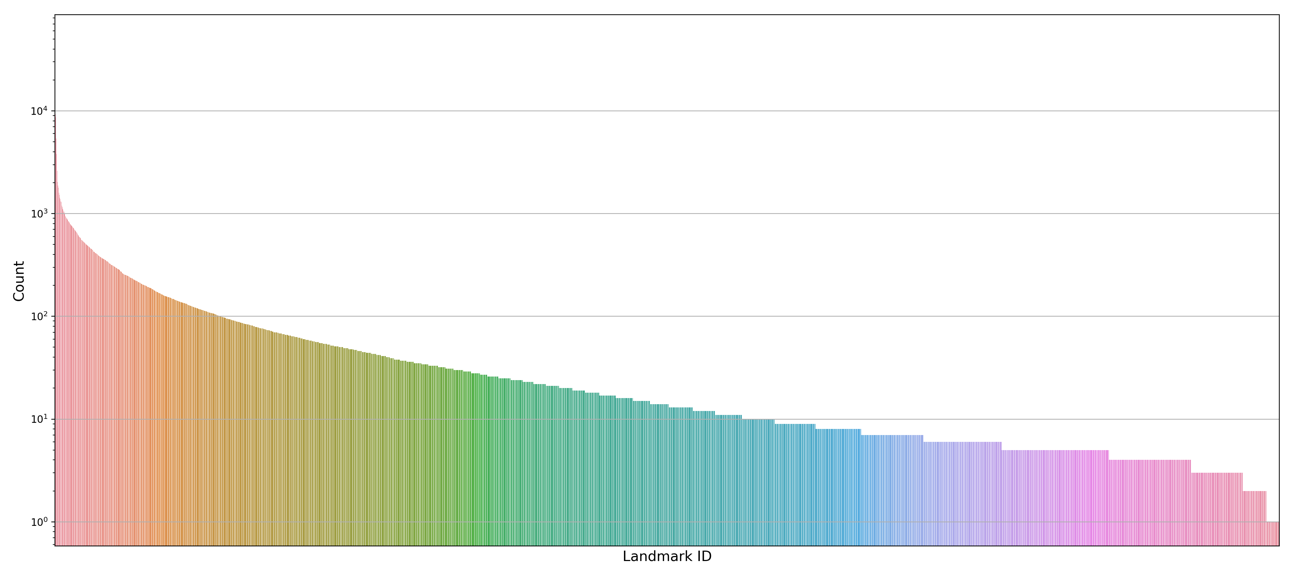
\includegraphics[width=1.0\linewidth]{./figures/all_distribution.png}
\caption{Count distribution of Google-Landmarks dataset}
\label{fig:all_distribution}
\end{figure}

Limited by the computation resources, in this work, only a subset of training images are used. More specifically, there are at most 10 training images kept for each landmark. Based on this criterion, 113,783 training images in 14,943 different landmarks are chosen as the training set. The count distribution is shown in Fig.~\ref{fig:subset_distribution}. In addition, 22,255 images with 7,675 different landmarks are chosen as the validation set and 22,391 images with 14,436 different landmarks are chosen as the test set.

% ---------------------------------------------------------------------
\begin{figure}[hbtp]
\centering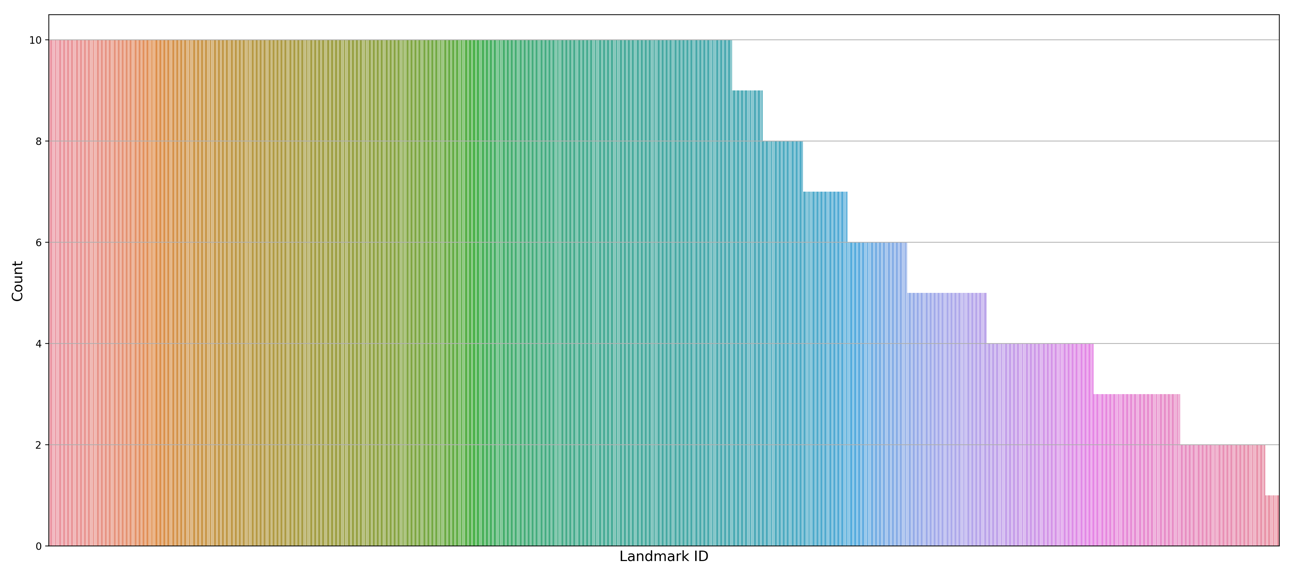
\includegraphics[width=1.0\linewidth]{./figures/subset_distribution.png}
\caption{Count distribution of training images}
\label{fig:subset_distribution}
\end{figure}


% ---------------------------------------------------------------------
\section{Methodology}
\label{S:method}

As discussed in Section~\ref{S:introduction}, with 14,943 different landmarks, classical multi-class classification networks which use fully-connected layer as the output layer are not appropriate. To solve this problem, this work focuses on metric learning. Through appropriate algorithms, the original images can be represented in a new space such that similar images will be close to each other while different images will have larger distance. Fig.~\ref{fig:triplet_learning} clearly shows this process.

% ---------------------------------------------------------------------
\begin{figure}[h]
\centering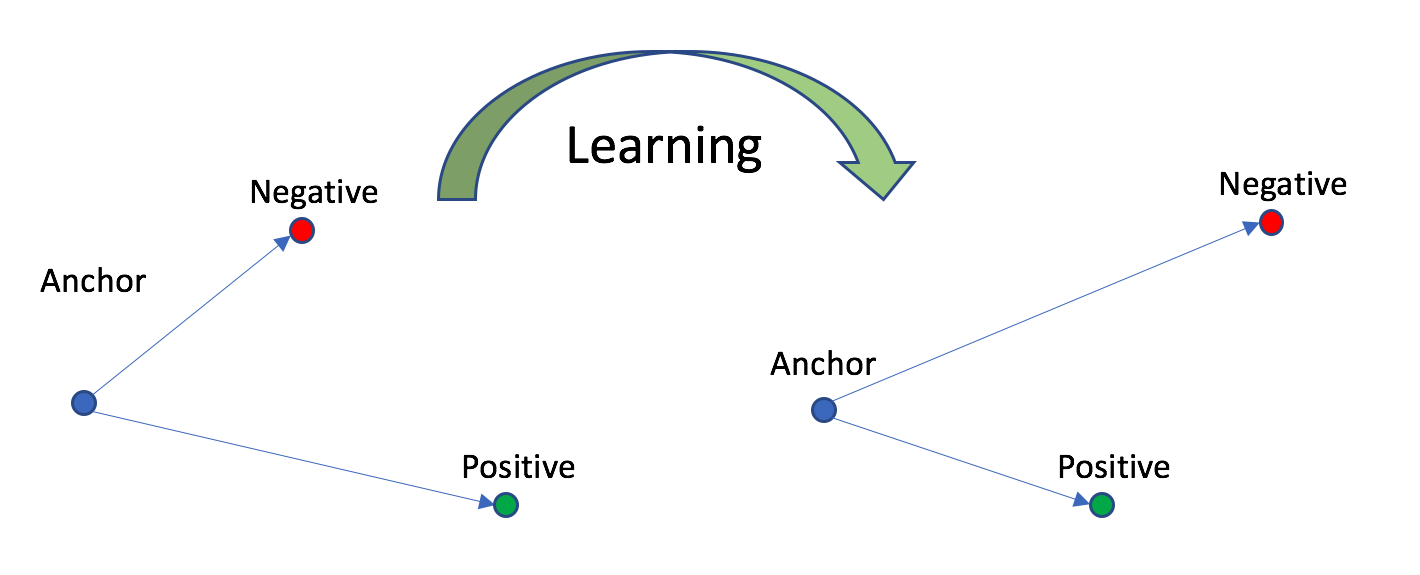
\includegraphics[width=0.8\linewidth]{./figures/learning.png}
\caption{Illustration of metric learning}
\label{fig:triplet_learning}
\end{figure}

Given an image (Anchor image) to determine the landmark it contains, there are two extra images used,  Positive image and Negative image. Positive image contains the same landmark with the Anchor image while Negative image contains different landmarks. When the system doesn't work correctly, the distance between the Anchor image and the Positive image would be larger than the distance between the Anchor image and the Negative image. Through metric learning, the system should be able to learn a metric such that the distance between the Anchor image and the Positive image is smaller than the distance between the Anchor image and the Negative image. In this way, the landmark of the Anchor image can be predicted using the landmarks from the closest images.

The idea in Fig.~\ref{fig:triplet_learning} leads to so-called triplet loss~\cite{schroff2015facenet}. Suppose the Anchor image, Positive image, and Negative image are denoted by $a$, $p$, and $n$, and the system defines some representation function $f(\cdot)$. Then the Euclidean distance between $a$ and $p$ is $||f(a) - f(p)||^2_2$ and the distance between $a$ and $n$ is $||f(a) - f(n)||^2_2$. Through training, the system should be able to distinguish positive and negative images such that:
\begin{equation}
||f(a) - f(p)||^2_2 <= ||f(a) - f(n)||^2_2
\end{equation}

To make the system more robust, some margin $\alpha$ is added such that:
\begin{equation}
||f(a) - f(p)||^2_2 + \alpha <= ||f(a) - f(n)||^2_2
\end{equation}

From above equations, triplet loss $L(a, p, n)$ is defined as:
\begin{equation}
L(a, p, n) = max\{||f(a) - f(p)||^2_2 + \alpha - ||f(a) - f(n)||^2_2, 0\}
\label{eq:triplet}
\end{equation}

The goal of the training is to minimize the triplet loss defined in Eq.~\ref{eq:triplet}. Based on above description, the corresponding triplet network architecture is described in Fig.~\ref{fig:system}.

% ---------------------------------------------------------------------
\begin{figure}[h]
\centering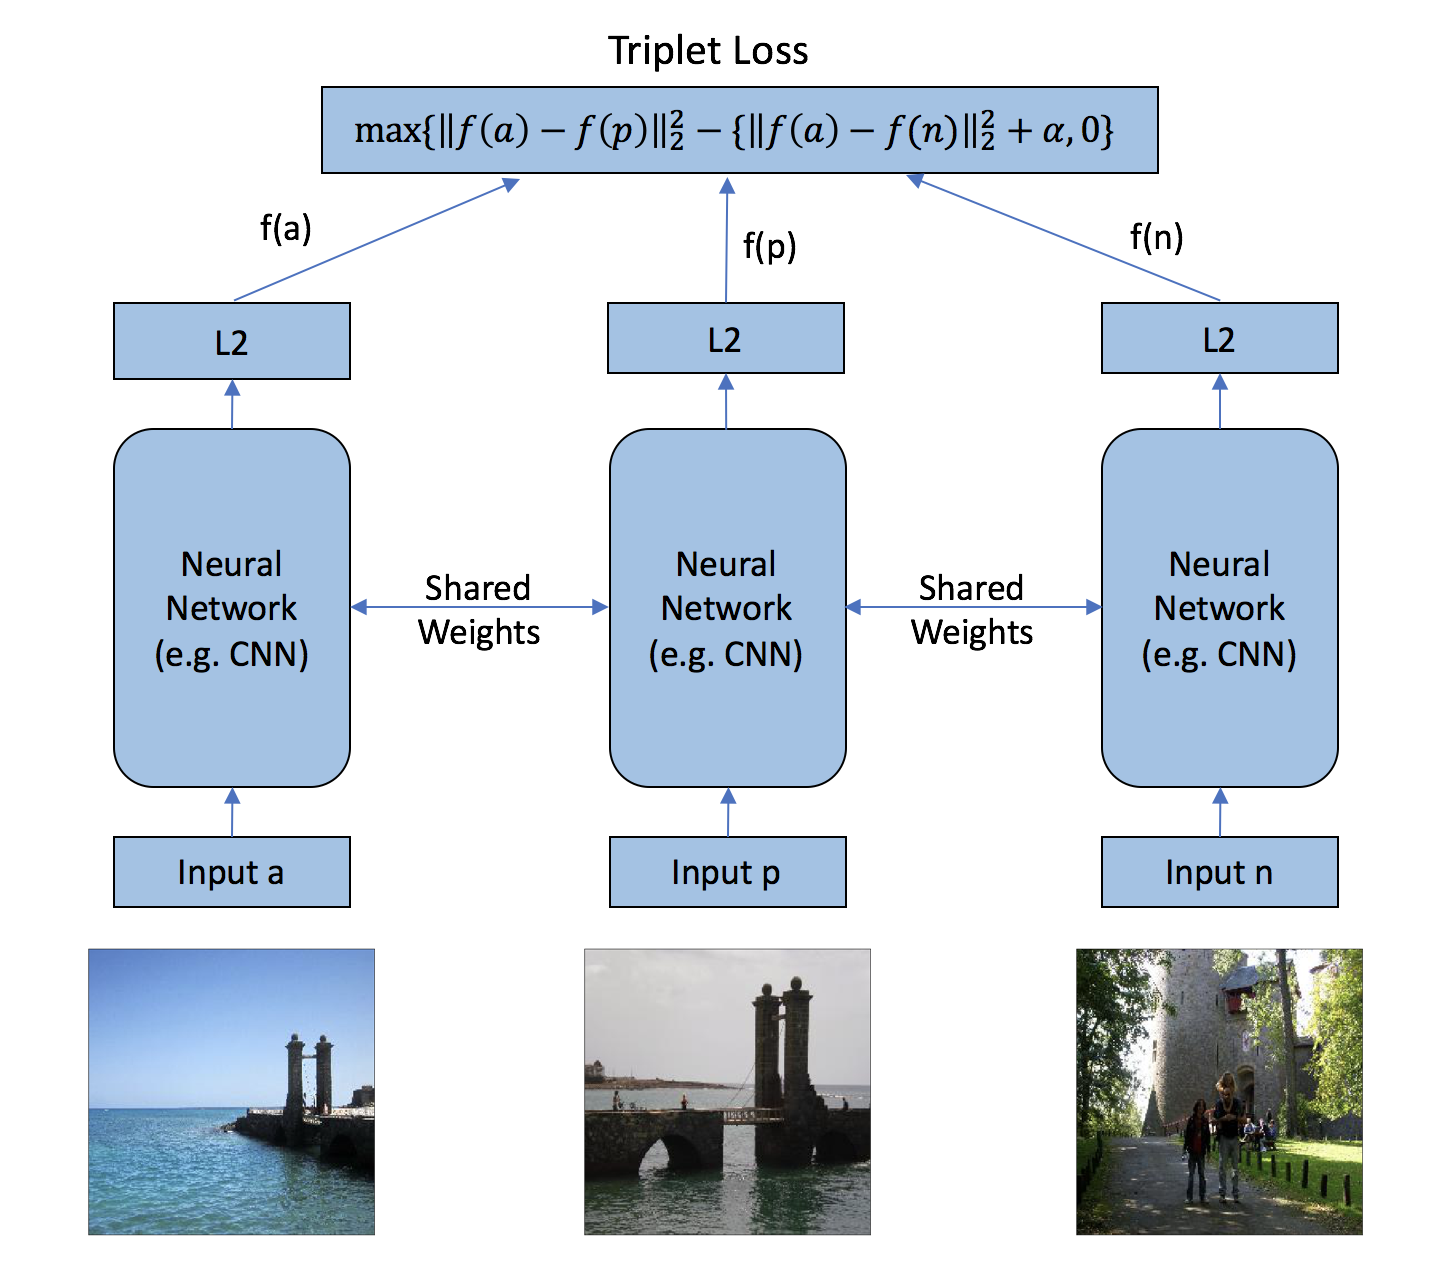
\includegraphics[width=0.85\linewidth]{./figures/triplet.png}
\caption{Triplet network overall architecture}
\label{fig:network}
\end{figure}

In Fig.~\ref{fig:network}, there are three images $a$, $p$, and $n$ as the input images. The input images are first processed by the same base-network. For computer vision tasks, CNN is generally used as the base-network. To define appropriate distance functions, the output from the base-network is normalized using L2 normalization. Finally, the triplet loss is computed using Eq.~\ref{eq:triplet}. The whole network is optimized using backpropagation. The whole system is implemented using Keras with TensorFlow as backend and all the code is available in GitHub: \textit{https://github.com/JifuZhao/Landmark-Recognition}.

As shown in Fig.~\ref{fig:network}, the performance of the whole system is determined by the base-network. Building a CNN from scratch is suggested when there are enough training images and advanced hardware. However, in this paper, limited by computation resources, building base-network from scratch is not appropriate. In addition to building CNN from scratch, pretrained CNNs can also be utilized. The simplest way is to directly apply the pretrained CNNs on landmark recognition problem without training. Since the base-network is not optimized for landmark recognition, the performance of the system is limited. Another choice is to fine-tune the pretrained CNNs. For pretrained CNNs, the lower convolution layers are usually assumed to encode more generic and reusable features, while the higher convolution layers encode specialized features~\cite{chollet2017deep}. Based on this idea, during training process, the weights for lower layers will be frozen and only the weights for higher layers are trained. Through backpropagation, the pretrained CNNs can be further optimized for landmark recognition.

Figure~\ref{fig:network} depicts the training process for base-network. With the base-network, the next step is to determine the landmark for unseen images. Given a large number of training images that contain different landmarks, for the unseen images, this turns out to be finding the most similar images such that the landmark for unseen images are inferred by the most similar images, which can be solved using k-nearest neighbor (KNN) algorithm. The whole system is shown in Fig.~\ref{fig:system}.

% ---------------------------------------------------------------------
\begin{figure}[hbtp]
\centering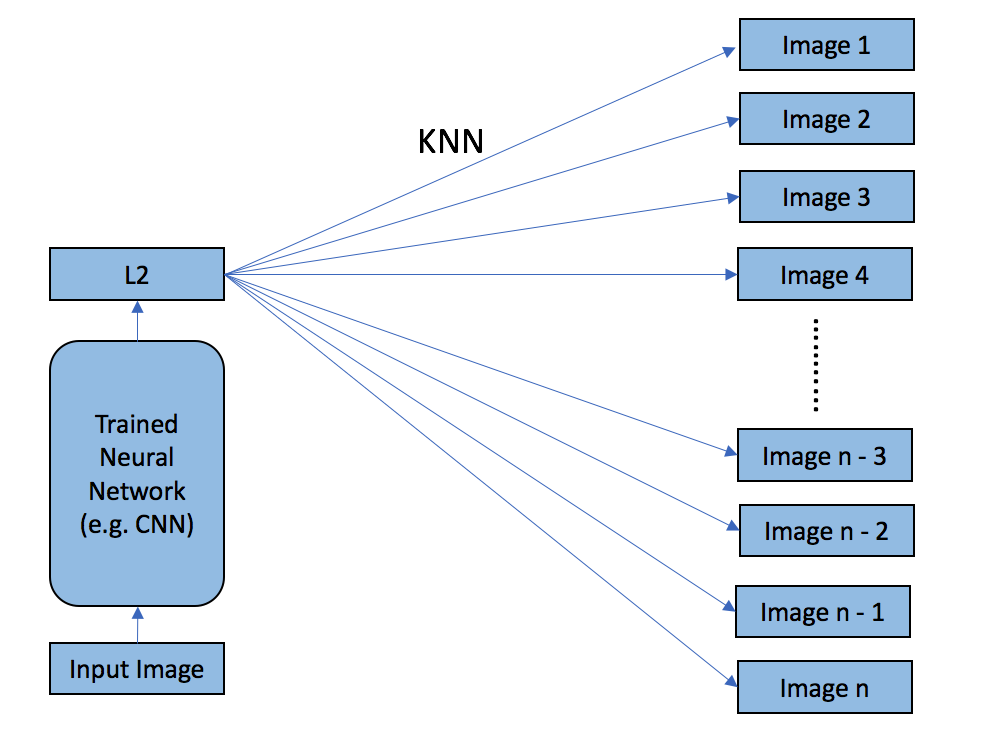
\includegraphics[width=0.8\linewidth]{./figures/system.png}
\caption{Overall landmark recognition system architecture}
\label{fig:system}
\end{figure}

In Fig.~\ref{fig:system}, given a new input image, the pretrained neural network will compute its representation in a new space. Through KNN algorithm, the system will find the most similar images in the reference image pool and make prediction based on the retrieved images.

% ---------------------------------------------------------------------
\section{Results}
\label{S:result}

As discussed in Section~\ref{S:method}, this paper implements two types of pretrained CNNs: naive implementation and fine-tuning. More specifically, VGG16 and InceptionV3 models pretrained on ImageNet dataset are implemented. Fig.~\ref{fig:accuracy} shows the performance of different algorithms. VGG16 only and InceptionV3 only models implement pretrained VGG16 and InceptionV3 without further training, while VGG16 triplet and InceptionV3 triplet models are the models with fine-tuning. As a comparison, Fig.~\ref{fig:accuracy} also shows the result of random guess. It is clear that, as the number of retrieved images increases, the accuracy also increases. The best top-1 accuracy is from InceptionV3 triplet model, which gives $47\%$ top-1 accuracy.

% ---------------------------------------------------------------------
\begin{figure}[h]
\centering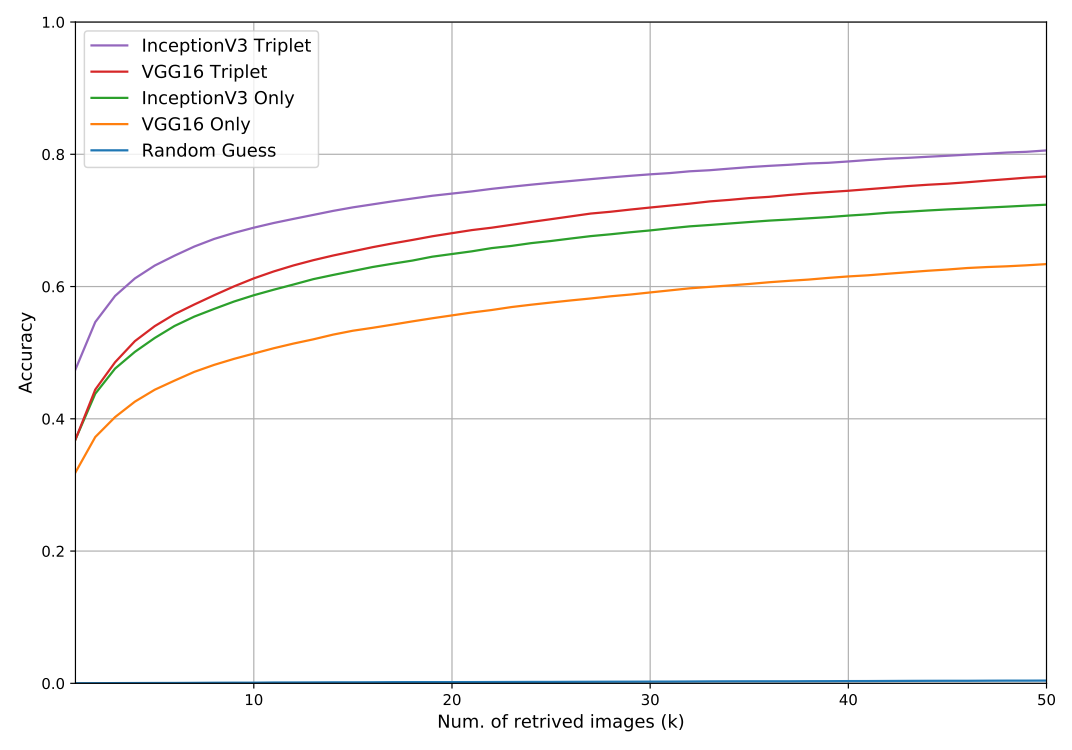
\includegraphics[width=0.7\linewidth]{./figures/accuracy.png}
\caption{Top-k image retrieval accuracy for different numbers of retrieved images}
\label{fig:accuracy}
\end{figure}

To show the retrieved results of the model, Fig.~\ref{fig:result} shows the top-6 retrieved images for randomly sampled 5 images with InceptionV3 triplet model. From Fig.~\ref{fig:result}, for some images, the built system can accurately predict the landmarks for the unseen images. However, for some unseen images, the system cannot make accurate prediction based on most similar images.

% ---------------------------------------------------------------------
\begin{figure}[h]
\centering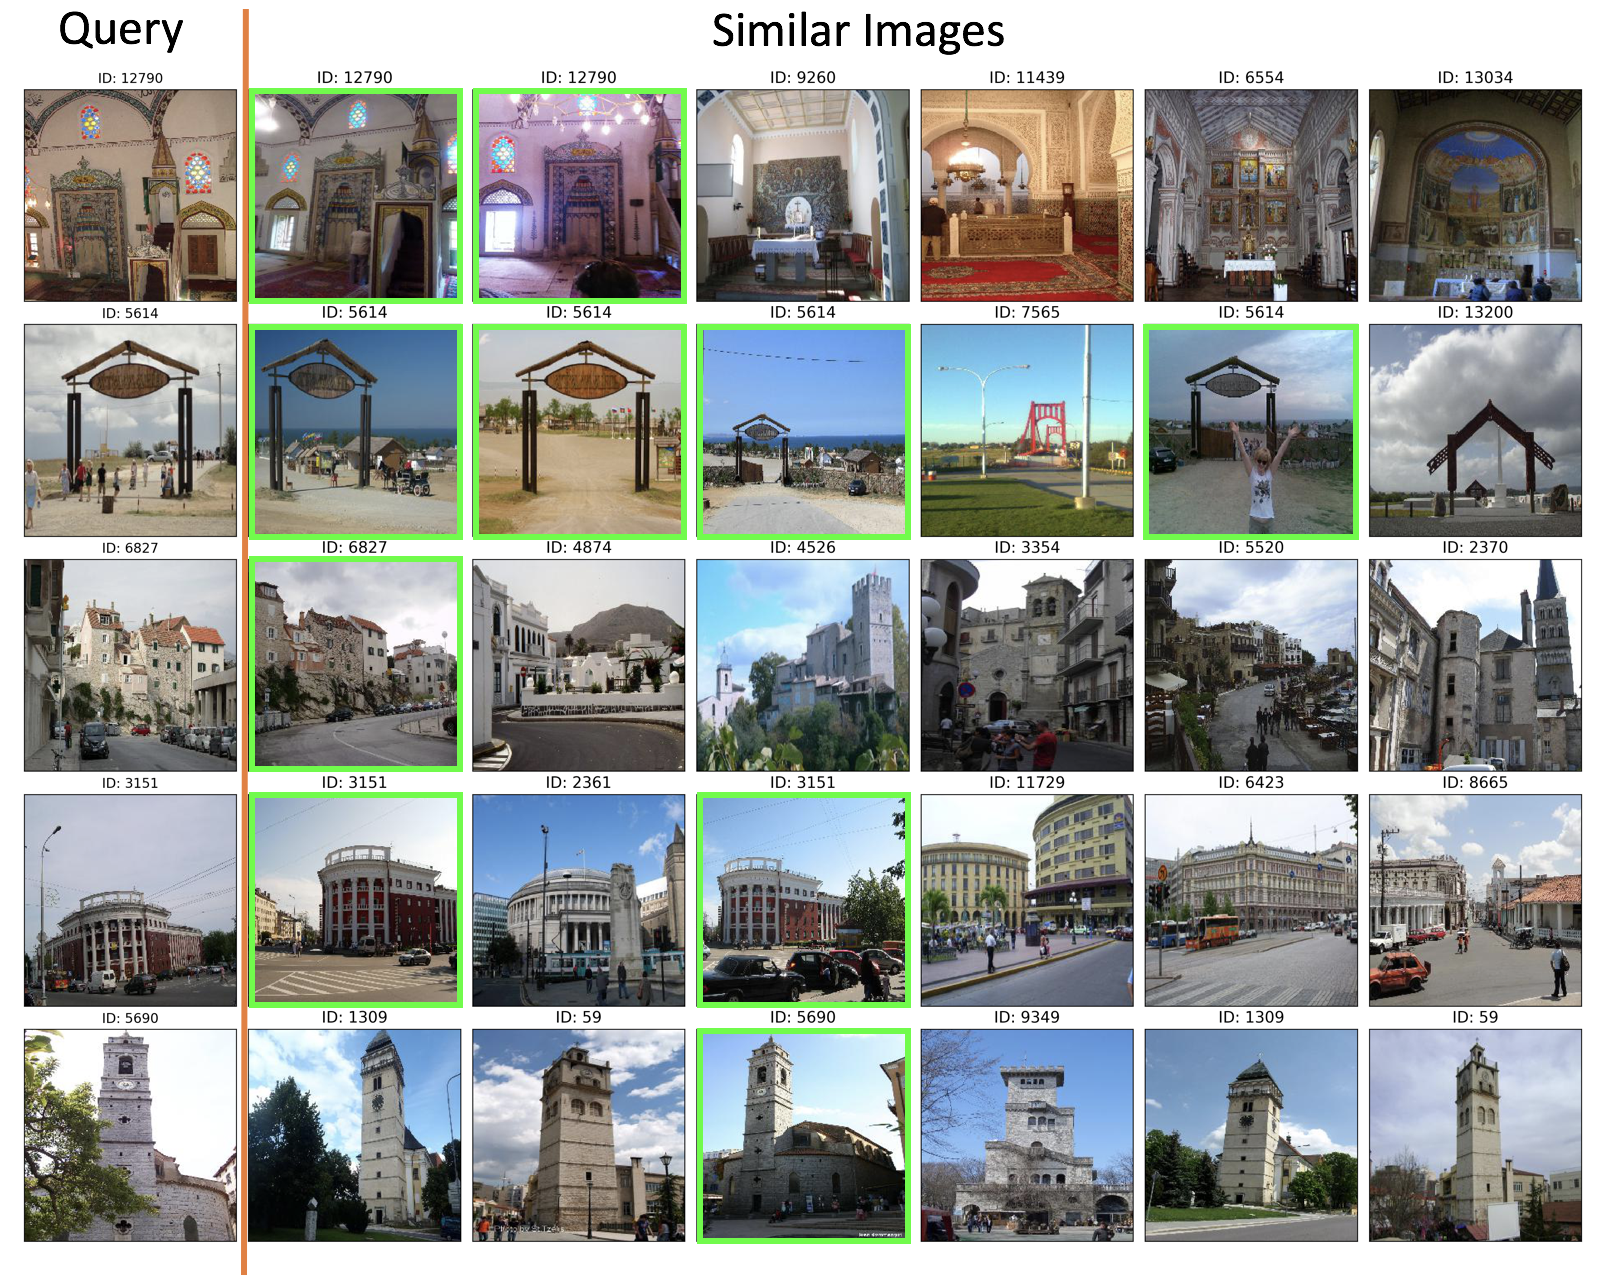
\includegraphics[width=1.0\linewidth]{./figures/result.png}
\caption{Top-6 image retrieval results from sample query images}
\label{fig:result}
\end{figure}

% ---------------------------------------------------------------------
\section{Conclusion}
\label{S:conclusion}

This paper studies one specific one-shot learning problem, landmark recognition. Considering the object recognition as a metric learning problem, this paper implements triplet network and fine-tunes pretrained CNN models to extract useful features from the original images. With KNN algorithm, this paper achieved $47\%$ top-1 accuracy on separate test dataset.

However, there are further procedures to improve the performance of the system. As discussed in Section~\ref{S:data}, the input images are pretty noisy. Through image processing, for example, adjusting the image such that the landmarks are at the center of the images and irrelevant objects are removed, the performance of the system might be further improved. In addition, due to computation resource limitation, currently, only less than $10\%$ of the total training images are actually used and the structure of the base-network hasn't been explicitly explored. All these factors might influence the performance of the system. The future work will focus on processing the input images and exploring better base-networks.

% ---------------------------------------------------------------------\
%\bibliographystyle{model1-num-names}
%\nocite{*}

\bibliographystyle{unsrt}
\section{\refname}

\bibliography{reference.bib}

\end{document}

%%
%% End of file `elsarticle-template-1-num.tex'.